\documentclass[10pt,pdf,hyperref={unicode}]{beamer}

\usepackage[utf8]{inputenc}
\usepackage[russian]{babel}
\usepackage{amssymb,amsmath}
\textwidth=10.7cm % ширина текста


\usepackage{color}
\usepackage{url}

\usepackage{indentfirst}
\usepackage{graphicx}

\usetheme{Warsaw}%Goettingen}


\title{Построение ансамбля алгоритмов рекомендаций}
\subtitle{Выпускная квалификационная работа}

%\author{Кудрявцев Георгий}
\institute{\begin{flushright}
      \parbox{0.5\textwidth}{
        \raggedleft
        \textbf{Выполнил:}\\
        студент 417 группы\\
        Кудрявцев Георгий Алексеевич\\[5mm]
        \textbf{Научный руководитель:}\\
        д.ф-м.н., профессор\\
        Дьяконов Александр Геннадьевич
      }
    \end{flushright}}
\date{2 июня 2016 г.}
\begin{document}
\frame{\titlepage}
%\AtBeginSection{
%    \begin{frame}
%        \frametitle{Содержание}
%        \tableofcontents[currentsection]
%        \end{frame}
%}

%\begin{frame}{Предметная область}
% Рассматривается задача ранжирования по данным с двоичной релевантностью.
% 
% На практике данная задача решается при помощи алгоритмов машинного обучения.
% 
% В данной работе рассматриваются факторизационные методы и их линейные ансамбли.
%\end{frame} 

\begin{frame}{Постановка задачи}
Задача ранжирования.

\bigbreak

Пусть есть некоторое множество пользователей и предметов, а также множество пар, состоящих из одного пользователя и предмета.

 Для каждого пользователя необходимо предоставить список предметов в порядке убывания предпочтения.
\end{frame}

%\begin{frame}{Актуальность задачи}
%
%Построение рекоммендаций для:
%
%\begin{itemize}
%\item социальных сетей
%
%\item сайтов знакомств
%
%\item интернет магазинов
%\end{itemize}
%\end{frame}

\begin{frame}{Цель и задачи}
%Составить обзор современных факторизационных методов ранжирования и экспериментально сравнить их эффективность на различных наборах данных, а также предложить метод ансамблирования, который стабильно улучшает качество ранжирования.



\begin{itemize}
\item Реализовать современные факторизационные методы ранжирования,  а также экспериментально сравнить их на реальных данных. 

\item Исследовать способы ансамлирования предыдущих методов и экспериментально сравнить их на реальных данных.
\end{itemize}

\end{frame}







\begin{frame}{Набор данных}

%\textbf{Входные данные}:
	Набор данных представлен в виде множества пар \\(пользователь, предмет). Cчитается, что в этих парах пользователь взаимодействовал с предметом. Например, пользователь u покупал товар i.
	\bigbreak
 Матрица $R$ размера $M \times N$, где $M$ - количество пользователей, $N$ - количество предметов. $R_{ui}$ = 1, если пользователей $u$ взаимодействовал с предметом $i$.
 
  В противном случае $R_{ui}$ = 0.

%\textbf{Выходные данные}: 
%
%Для каждого пользователя $u$ ранжированный список предметов, которые не лежат в тренировочной выборке.
\end{frame}

\begin{frame}{Факторизационные методы}

\begin{figure}[h]
\center{\includegraphics[width=0.9\linewidth]{Factorizationmatrix}}
%\caption{Идея факторизационного метода}
\label{pic:latexpic}
\end{figure}

\begin{center}
$R_{ui} \approx f_{ui} = \langle P_u, Q_i \rangle$
\end{center}

\begin{center}
K  - размерность латентного пространства.
\end{center}
\end{frame}


\begin{frame}{Cуществующие методы}

\begin{itemize}
\item \textbf{CLiMF}\footnote{Yue Shia, Alexandros Karatzogloub, Linas Baltrunas.
CLiMF: learning to maximize reciprocal rank with collaborative less-is-more filtering. 2012}
 -- Факторизационный метод, который оптимизирует сглаженную версию метрики MRR.
  	
\item \textbf{BPR\_MF}\footnote{Steffen Rendle, Christoph Freudenthaler, Zeno Gantner.    
         BPR: Bayesian Personalized Ranking from Implicit Feedback. 2009}
-- Факторизационный метод, который оптимизирует AUC.
\item \textbf{TFMAP}\footnote{Yue Shia,Alexandros Karatzogloub, Linas Baltrunas.
TFMAP: Optimizing MAP for Top-N Context-aware Recommendation. 2012} 
-- Факторизационный метод, который оптимизирует сглаженную метрику MAP.
\item \textbf{iMF}\footnote{Yifan Hu, Yehuda Koren, Chris Volinsky.
	Collaborative Filtering for Implicit Feedback Datasets. 2008}
-- Факторизационный метод, который оптимизирует взвешенную квадратичную ошибку.
\end{itemize}
\end{frame}

%\begin{frame}{Пример функционала качества}
%MAP -- 	Mean Average Precision
%	
%	
%	\begin{equation*}
%	\begin{split}
%	 & AP@n(u) = \frac{1}{n}\sum_{k=1}^n rel(u, k) P@k(u)  \\
%	 & MAP@n = \frac{1}{M}\sum_{k=1}^M AP@n(u) \\
%	\end{split}			
%	\end{equation*}
%\end{frame}

\begin{frame}{Сравнение методов}

\begin{table}[H]
\begin{flushleft}
\resizebox{0.6\textwidth}{!}{\begin{minipage}{\textwidth}
\begin{tabular}{|c|c|c|c|c|c|c|c|c|c|c|}
\hline
\multicolumn{11}{|c|}{MovieLens 100k}\\
\hline
& \multicolumn{5}{|c|}{n = 10} & \multicolumn{5}{|c|}{n = 5}\\
\hline
   & PopRec & CLiMF & BRP\_MF & iMF & TFMAP & PopRec & CLiMF & BRP\_MF & iMF & TFMAP  \\
\hline
P@5 &0.1399 & 0.1429 & 0.2672 &	\textbf{0.2972} & 0.1478 & 0.2401 & 0.2468 &	0.3945 & \textbf{0.4476} & 0.257 \\
\hline
1call@5 & 0.4516 & 0.4565 & 0.6947 & \textbf{0.7332} & 0.4354 &  0.6625 & 0.6550 & 0.8461 & \textbf{0.8883} &	0.6153\\
\hline
NDCG@5 & 0.1549 & 0.1592 & 0.2837 & \textbf{0.3220} & 0.1652 & 0.2591 & 0.2611 &	0.4118 & \textbf{0.4782} & 0.2748\\
\hline
MAP@5 & 0.2853 & 0.2934 & 0.4511 & \textbf{0.5043}  & 0.2882 &  0.4245 &	0.4179 & 0.5815 & \textbf{0.6651} & 0.4169\\
\hline
MRR & 0.3413& 0.3451 & 0.5025 & \textbf{0.5568} & 0.3384 &  0.4806 & 0.4711 &0.6335 & \textbf{0.7205} & 0.4624\\
\hline
AUC & 0.8597 & 0.8470 & \textbf{0.9317} & 0.9310 & 0.8503 & 0.8566 &	0.8417 & \textbf{0.9290} & 0.9283 & 0.8471\\
\hline
\multicolumn{11}{|c|}{Epinion}\\
\hline
& \multicolumn{5}{|c|}{n = 10} & \multicolumn{5}{|c|}{n = 5}\\
\hline
   & PopRec & CLiMF & BRP\_MF & iMF & TFMAP & PopRec & CLiMF & BRP\_MF & iMF & TFMAP  \\
\hline
P@5 & 0.0301 & 0.0294 &	0.0557 & \textbf{0.06940} &	0.0273 & 0.0564 & 0.0545 &	0.0999 & \textbf{0.1248} & 0.0548 \\
\hline
1call@5 & 0.1327 & 0.1300 &	0.2267 & \textbf{0.2726} & 0.1213 & 0.2301 & 0.2237 & 0.3532	 & |\textbf{0.4251} & 	0.2221\\
\hline
NDCG@5 & 0.0338 &	0.0332 & 0.0586 &  \textbf{0.0742} & 0.0312 & 0.0636 & 0.0619 &	0.1052 & \textbf{0.1316} &	0.0628 \\
\hline
MAP@5 &  0.0767 & 0.0757 & 0.1210 &	\textbf{0.1515} & 0.0716 &  0.1375 &	0.1353 & 0.1973	& \textbf{0.2438} & 0.1363 \\
\hline
MRR & 0.0999 & 0.0990 &	0.1541 & \textbf{0.1864} & 0.0946 & 0.1703 &	0.1680 & 0.2385 &  \textbf{0.2853} &	0.1687\\
\hline
AUC &0.8690 &  0.7685 &	\textbf{0.9192} & 0.9175 & 0.8607 &  0.8700 & 0.7576 & \textbf{0.9185} & 0.9159 &	0.8615\\
\hline
\end{tabular}
\end{minipage}}
\end{flushleft}
\end{table}

\end{frame}

\begin{frame}{Сравнение методов}

\begin{table}[H]
\begin{flushleft}
\resizebox{0.6\textwidth}{!}{\begin{minipage}{\textwidth}
\begin{tabular}{|c|c|c|c|c|c|c|c|c|c|c|}
\hline
\multicolumn{11}{|c|}{Slashdot}\\
\hline
& \multicolumn{5}{|c|}{n = 10} & \multicolumn{5}{|c|}{n = 5}\\
\hline
   & PopRec & CLiMF & BRP\_MF & iMF & TFMAP & PopRec & CLiMF & BRP\_MF & iMF & TFMAP  \\
\hline
P@5 & 0.0154 & 0.0154 & 0.0247 & \textbf{0.0393} & 0.0139 & 0.0294 &	0.0295 & 0.0420 & \textbf{0.0722} & 0.0289 \\
\hline
1call@5 & 0.0721 & 0.0725 &	0.1045 & \textbf{0.1582} & 0.0662 & 0.1307 &  0.1322 & 0.1608 & \textbf{0.2626} &	0.1295\\
\hline
NDCG@5 & 0.0179 & 0.0179 & 0.0265 &	\textbf{0.0430} & 0.0144 & 0.0335 &	0.0334 & 0.0439 & \textbf{0.0781} & 0.0324 \\
\hline
MAP@5 & 0.0428 & 0.0427 & 0.0566 & \textbf{0.0901} &	0.0325 & 0.0764 & 0.0764 & 0.0867 &	\textbf{0.1522} & 0.0738\\
\hline
MRR &  0.0597 &	0.0589 & 0.0775 & \textbf{0.1151} & 0.0490 & 0.1024 & 0.1013 & 0.1150 & \textbf{0.1864} &	0.0989\\
\hline
AUC & 0.8457 & 0.7213 & \textbf{0.8710} & 0.8703 &  0.8376 &  0.8460 & 0.7073 &	0.8631 & \textbf{0.8665} & 0.8354\\
\hline
\multicolumn{11}{|c|}{Movielens 1m}\\
\hline
& \multicolumn{5}{|c|}{n = 10} & \multicolumn{5}{|c|}{n = 5}\\
\hline
   & PopRec & CLiMF & BRP\_MF & iMF & TFMAP & PopRec & CLiMF & BRP\_MF & iMF & TFMAP  \\
\hline
P@5 & 0.1336 & 0.1157 &	0.2237 & \textbf{0.2600} & 0.0792 &  0.2265 & 0.212507 & 0.3345 & \textbf{0.3972} & 0.1405 \\
\hline
1call@5 & 0.4112 & 0.3692 &	0.6141 & \textbf{0.6520} & 0.2870 & 0.5779 & 0.5595 & 0.7531 & \textbf{0.8010} & 0.4420\\
\hline
NDCG@5 & 0.1439 & 0.1198 & 0.2400 &	\textbf{0.2799} & 0.0838 & 0.2387 &	0.2181 & 0.3501 & \textbf{0.4175} & 0.1504\\
\hline
MAP@5 & 0.2564 & 0.2091 & 0.3942 &	\textbf{0.4424} & 0.1603 &  0.3780 &  0.3399 & 0.5085 &	\textbf{0.5767} & 0.2689\\
\hline
MRR &  0.3780 &	0.3399 & 0.5085 & \textbf{0.5767} & 0.2689 & 0.4189 & 0.3856 & 0.5588 & \textbf{0.6255} & 0.3142\\
\hline
AUC & 0.8573 & 0.8489 &	\textbf{0.9244} & 0.9171 & 0.8491 &  0.8579 & 0.8523 & \textbf{0.9228} & 0.9157 &	0.8502\\
\hline
\end{tabular}
\end{minipage}}
\end{flushleft}
\end{table}

\end{frame}



\begin{frame}{Линейный ансамбль}
Пусть имеется множество базовых алгоритмов $b_i(x)$. 

\bigbreak

Необходимо подобрать такие веса $\alpha_i$, чтобы линейная комбинация алгоритмов $\hat{b}(x) = \sum_i \alpha_i b_i(x)$ показывала лучший результат по какому-нибудь заданному функционалу. 
\end{frame}

\begin{frame}{Способы построения линейного ансамбля}

\begin{itemize}
\item Простое голосование

\item Линейная регрессия

\item Оптимальное взвешенное голосование
\end{itemize}

\end{frame}

\begin{frame}{Оптимальное взвешенное голосование}

 Рассмотрим линейную комбинацию двух алгоритмов ранжирования  в следующем виде:
\begin{equation*}
	\hat{f}_{ui} = \alpha f_{ui}^{m_1} + (1 - \alpha) f_{ui} ^ {m_2} \textrm{\ , где $0 \leq \alpha \leq 1$}
\end{equation*} 
	
\begin{figure}[h]
\center{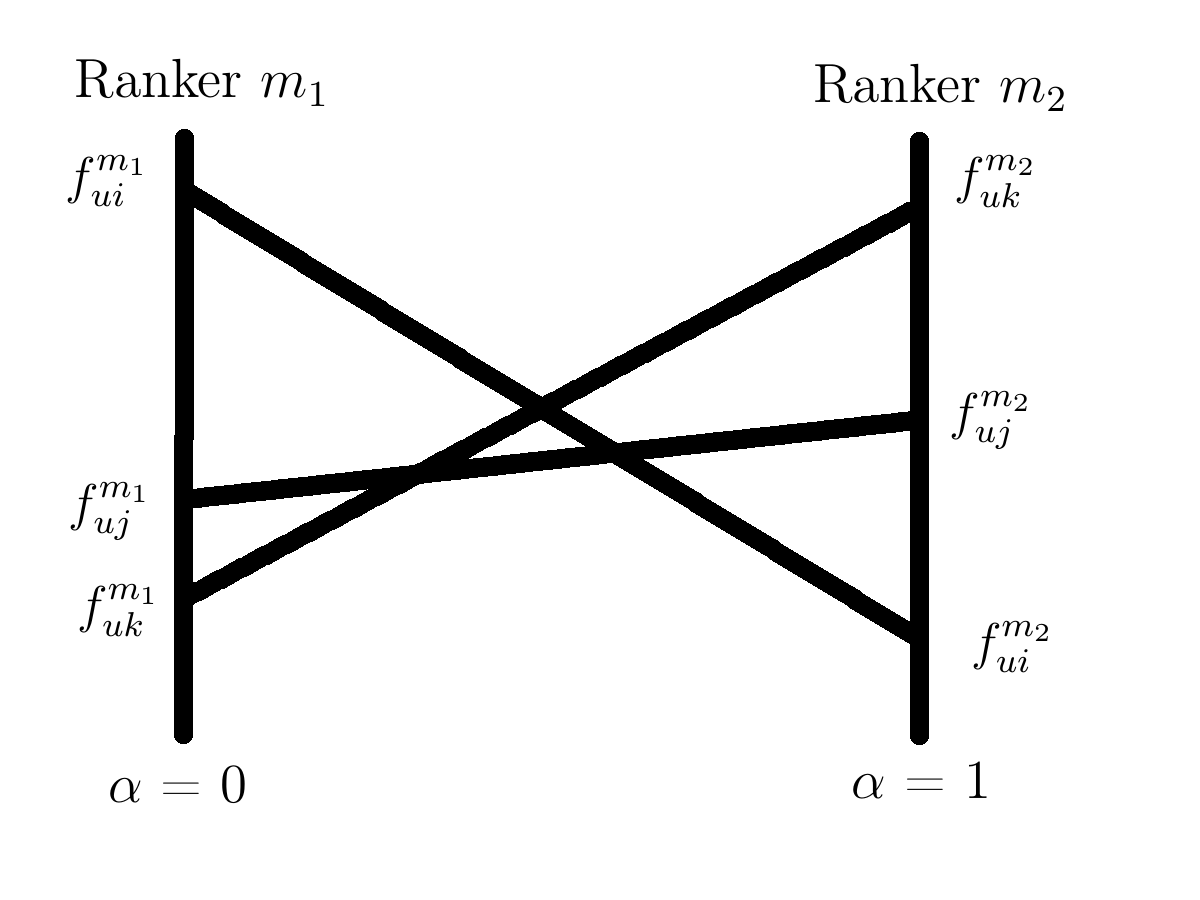
\includegraphics[width=0.4\linewidth]{latexpic}}
\caption{Графическая демонстрация идеи метода \footnote{Qiang Wu, Christopher J. C. Burges, Krysta M. Svore.	 Adapting Boosting for Information Retrieval Measures. 2010.}}
\label{pic:latexpic}
\end{figure}

\end{frame}

\begin{frame}{Оптимальное взвешенное голосование}
Пусть $b_i$ базовые методы ранжирования,

($b_i$, $b_j$) - оптимальное взвешенное голосование.

\bigbreak
Стратегии построения ансамбля для 4 методов:

\begin{itemize}
\item бустинг -- $(((b_{i_1}, b_{i_2}), b_{i_3}), b_{i_4})$
\item дерево -- $((b_{i_1}, b_{i_2}), (b_{i_3}, b_{i_4}))$
\end{itemize}

\end{frame}

\begin{frame}{Сравнение ансамблей}

\begin{table}[H]
\begin{flushleft}
\resizebox{0.7\textwidth}{!}{\begin{minipage}{\textwidth}
\begin{tabular}{|c|c|c|c|c|c|c|c|c|c|c|}
\hline
 \multicolumn{11}{|c|}{MovieLens 100k} \\
\hline
& \multicolumn{5}{|c|}{ptest = 10\%, pvalid=10\%, maxiter = 5} & \multicolumn{5}{|c|}{ptest = 20\%, valid = 10\%, maxiter = 5}\\
\hline
  & BSM  & SV &  RV & OVB & OVT &BSM  & SV & RV & OVB & OVT \\
\hline
P@5 & 0.2965 & 0.1602 &	0.2528 & \textbf{0.3069} & 0.3019 & 0.4451 &	0.2531 & 0.3831 & \textbf{0.4498} & 0.4464 \\
\hline
1call@5 & 0.7344 & 0.4950 & 0.6712 & \textbf{0.7580} & 0.7555 & 0.8706 & 0.6203 & 0.8039 &	\textbf{0.8784} & 0.8734\\
\hline
NDCG@5 &0.3201 & 0.1778 & 0.2783 & \textbf{0.3307} &	0.3257 & 0.4705 & 0.2738 & 0.4070 &	\textbf{0.4770} & 0.4752\\
\hline
MAP@5 & 0.5035 & 0.3239 & 0.4599 & \textbf{0.5185} & 0.5152 & 0.6480 & 0.4261 & 0.5763 &	0.6555 & \textbf{0.6562}\\
\hline
 \multicolumn{11}{|c|}{Epinion} \\
\hline
& \multicolumn{5}{|c|}{ptest = 10\%, pvalid=10\%, maxiter = 5} & \multicolumn{5}{|c|}{ptest = 20\%, valid = 10\%, maxiter = 5}\\
\hline
  & BSM  & SV &  RV & OVB & OVT &BSM  & SV & RV & OVB & OVT \\
\hline
P@5 & 0.0716 & 0.0295 &	0.0534 & \textbf{0.0764} & 0.0760 & 0.1283 &	0.0550 & 0.1000 & 0.1328 & \textbf{0.1363} \\
\hline
1call@5 &0.2710 & 0.1303 & 0.2183 &	\textbf{0.2921} & 0.2908 & 0.4179 & 0.2242 &	0.3595 & 0.4372 & \textbf{0.4438}\\
\hline
NDCG@5 &0.0775  & 0.0334 & 0.0572 &	\textbf{0.0830} & 0.0822 &  0.1384 &	0.0615 & 0.1062 & 0.1425 &	\textbf{0.1468}\\
\hline
MAP@5 & 0.1561 & 0.0759 & 0.1193 & \textbf{0.1688} & 0.1672 & 0.2536 & 0.1316 & 0.2035 & 0.2607 & \textbf{0.2686}\\
\hline
\end{tabular}
\end{minipage}}
\end{flushleft}
\end{table}

\end{frame}

\begin{frame}{Сравнение ансамблей}

\begin{table}[H]
\begin{flushleft}
\resizebox{0.7\textwidth}{!}{\begin{minipage}{\textwidth}
\begin{tabular}{|c|c|c|c|c|c|c|c|c|c|c|}
\hline
 \multicolumn{11}{|c|}{Slashdot} \\
\hline
& \multicolumn{5}{|c|}{ptest = 10\%, pvalid=10\%, maxiter = 5} & \multicolumn{5}{|c|}{ptest = 20\%, valid = 10\%, maxiter = 5}\\
\hline
  & BSM  & SV &  RV & OVB & OVT &BSM  & SV & RV & OVB & OVT \\
\hline
P@5 & 0.0431 & 0.0186 &	0.0291 & \textbf{0.0438} & 0.0436 &  0.0746 & 0.0362 & 0.0519 &	0.0757 & \textbf{0.0758}\\
\hline
1call@5 & 0.1644 & 0.0866 & 0.1272 & \textbf{0.1683} & 0.1671 & 0.2570 & 0.1577 & 0.2038 & 0.2631 & \textbf{0.2653} \\
\hline
NDCG@5 & 0.0473 & 0.0201 &	0.0312 & \textbf{0.0481} & \textbf{0.0481} & 0.0803 &	0.0397 & 0.0556 & 0.0819 & \textbf{0.0822}\\
\hline
MAP@5 & 0.0959 & 0.0455 & 0.0684 & 0.0976 & \textbf{0.0978} & 0.1506 & 0.0877 & 0.1140 & 0.1550 & \textbf{0.1562}\\
\hline
 \multicolumn{11}{|c|}{Movie Lens 1m} \\
\hline
& \multicolumn{5}{|c|}{ptest = 10\%, pvalid=10\%, maxiter = 5} & \multicolumn{5}{|c|}{ptest = 20\%, valid = 10\%, maxiter = 5}\\
\hline
  & BSM  & SV &  RV & OVB & OVT &BSM  & SV & RV & OVB & OVT \\
\hline
P@5 & 0.2601 & 0.1065 &	0.2374 & 0.2628 & \textbf{0.2639} &  0.3936 & 0.1974 & 0.3616 &	\textbf{0.3983} & 0.3944\\
\hline
1call@5 & 0.6541 & 0.3424 & 0.6186 & 0.6566 & \textbf{0.6593} & 0.7985 & 0.5255 & 0.7714 & \textbf{0.8075} & 0.8066\\
\hline
NDCG@5 & 0.2795 & 0.1104 & 0.2476 &	0.2830 & \textbf{0.2836} & 0.4127 &	0.2007 & 0.3710 & \textbf{0.4192} & 0.4157\\
\hline
MAP@5 & 0.4384& 0.1936 & 0.3859 & 0.4440 & \textbf{0.4438} & 0.5729 & 0.3127 & 0.5166 & \textbf{0.5839} & 0.5822\\
\hline

\end{tabular}
\end{minipage}}
\end{flushleft}
\end{table}

\end{frame}



\begin{frame}{Результаты работы}

\begin{enumerate}

\item Были реализованы основные факторизационные методы для задачи ранжирования для набора данных с двоичной релевантностью, а также было проведено их экспериментальное сравнение на различных наборах данных.

\item Предложена модификация оптимального взвешенного голосования, которая ускоряет его работу.

\item Все  факторизационные методы, ансамбли  и эксперименты, кроме линейной регрессии, были реализованы на языке python и C++.
\end{enumerate}

\end{frame}

\begin{frame}{Примеры метрик}

$rel(u, k)$ = 1, если предмет, стоящий на $k$ позиции в упорядоченном списке предметов для пользователя $u$, релевантен. 

В противном случае $rel(u, k)$ = 0. 

\bigbreak

\textbf{P@n} (Precision at n)

Определим для одного пользователя
	\begin{equation*}
		P@n(u) = \frac{1}{n}\sum_{k = 1}^n rel(u, k)
	\end{equation*}
	
\end{frame}

\begin{frame}{Примеры метрик}

\textbf{NDCG@n} (Normalized Discounted Cumulative Gain)
	
	Определим для одного пользователя
	
	\begin{equation*}
	\begin{split}
	 & G(u, k) = 2^{rel(u, k)} - 1 \\
	 & D(k) = \frac{1}{log_2(k + 1)} \\
	 & DCG@n(u) = \sum_{k=1}^n G(u, k) D(k) \\
	 & NDCG@n(u) = \frac{DCG@n(u)}{max DCG@n}
	\end{split}			
	\end{equation*}

\end{frame}

\end{document}





